\section{Overview of the Analyses}
\label{sec:analysis:demo_model}

\begin{figure}[hbt!]

\begin{tikzpicture}[->,>=stealth',shorten >=1pt,auto,  semithick, node distance=0.5cm]
\tikzstyle{section} = [state, rectangle, fill=gray!20]
\tikzstyle{result} = [state, rectangle, rounded corners]
\tikzstyle{auxresult} = [state,rectangle,draw=white]
\tikzstyle{input} = [state,rectangle, draw=blue, thick, fill=blue!20, align=center, rounded corners, minimum height=2em]
\tikzstyle{interresult} = [state, rectangle,dashed, rounded corners]

\node[section] (WCETANA)
   {
      \begin{tabular}{@{}c@{}}
         WCET\\
         Analysis\\
         (Section~\ref{fr:sec:analysis:wcet})
      \end{tabular}
   };


\node[auxresult] (SLOWFACTOR) [above right=of WCETANA,yshift=-20pt]
   {
      \begin{tabular}{@{}c@{}}
         Slowdown\\
         Factors
      \end{tabular}
   };

\node[result] (PROGWCET) [below right=of WCETANA,yshift=20pt]
   {
      \begin{tabular}{@{}c@{}}
         WCET of\\
         Programs
      \end{tabular}
   };


\node[interresult,node distance=2cm] (NOSHAREDWCET) [below =of WCETANA]
   {
      \begin{tabular}{@{}c@{}}
         Without Shared\\
         Variables
      \end{tabular}
   };

\node[result] (IMPACTWCET) [xshift=-1cm,yshift=-0.5cm, below right =of NOSHAREDWCET]
   {
      \begin{tabular}{@{}c@{}}
         Impact of\\
         Interference\\
         on WCET
      \end{tabular}
   };

\node[section,node distance=4cm] (HITMISSANA) [right =of WCETANA]
   {
      \begin{tabular}{@{}c@{}}
         Hit \& Miss\\
         Analysis\\
         (Section~\ref{fr:sec:cat_cache_access})
      \end{tabular}
   };

\node[input] (PARAMEDMODEL) [above =of HITMISSANA]
   {
      \begin{tabular}{@{}c@{}}
         Instantiated\\
         Model
      \end{tabular}
   };

\node[result] (INSTRACCU) [below left =of HITMISSANA,xshift=1cm]
   {
      \begin{tabular}{@{}c@{}}
         Instruction\\
         Accuracy
      \end{tabular}
   };

\node[auxresult] (MEMEACCU) [below right =of HITMISSANA,xshift=-1cm]
   {
      \begin{tabular}{@{}c@{}}
         Mem. Element\\
         Accuracy
      \end{tabular}
   };


\node[section] (INTERCAT) [right =of HITMISSANA,xshift=2.5cm]
   {
      \begin{tabular}{@{}c@{}}
         Interference\\
         Categorization\\
         (Section~\ref{fr:sec:analysis:exposing_interference})
      \end{tabular}
   };

\node[input] (PROTOCOL) [above =of INTERCAT]
   {
      \begin{tabular}{@{}c@{}}
         Cache Coherence\\
         Protocol
      \end{tabular}
   };

\node[interresult] (ANOTPROTO) [below =of INTERCAT]
   {
      \begin{tabular}{@{}c@{}}
         Annotated\\
         Protocol
      \end{tabular}
   };

\node[section] (INSTRIMPA) [below =of ANOTPROTO,xshift=-0.5cm]
   {
      \begin{tabular}{@{}c@{}}
         Instruction Impact\\
         Analysis\\
         (Section~\ref{fr:sec:analysis:missing_link})
      \end{tabular}
   };

\node[result] (RELINSTRINTER) [below =of INSTRIMPA]
   {
      \begin{tabular}{@{}c@{}}
         Relation Between\\
         Instruction \&\\
         Interference
      \end{tabular}
   };

\path[draw,->] (PARAMEDMODEL) -| (WCETANA);
\path[draw,->] ([yshift=-30pt]WCETANA) -- (PROGWCET);
\path[draw,->] ([yshift=30pt]WCETANA) -- (SLOWFACTOR);

\path[draw,->] (PARAMEDMODEL) -- (HITMISSANA);
\path[draw,->] (HITMISSANA) -- (INSTRACCU);
\path[draw,->] (HITMISSANA) -- (MEMEACCU);

\path[draw,->] (PROTOCOL) -- (INTERCAT);
\path[draw,->] (INTERCAT) -- (ANOTPROTO);
\path[draw,->] (ANOTPROTO) -- (INSTRIMPA);
\path[draw,->] (PARAMEDMODEL) -| ([xshift=10pt]INSTRIMPA.north west);
\path[draw,->] (INSTRIMPA) -- (RELINSTRINTER);

\path[draw,->] ([xshift=-20pt]WCETANA) -- ([xshift=-20pt]NOSHAREDWCET);
\path[draw,->] (PROGWCET) -- (IMPACTWCET);
\path[draw,->] (NOSHAREDWCET) -- (IMPACTWCET);
\end{tikzpicture}

\caption{Overview of Analyses in Chapter~\ref{cha:exposing_interference}}
\label{fig:analysis:summary}
\end{figure}

Figure~\ref{fig:analysis:summary} provides an overview of the analyses performed
in this chapter. Rectangles with a gray background correspond to analyses and
those without background are main results. Nodes without borders are auxiliary
results, meant to provide extra information. Rectangles with dashed borders are
intermediary results, which are not meant to be used on their own.

For the analyses presented in this chapter to provide relevant information to
the user, the model from Chapter~\ref{cha:modeling_cache_coherence} has to be
instantiated to match the user's chosen architecture (\textit{Instantiated
Model} in the figure). This instantiation corresponds to setting the model
parameters listed in Appendix~\ref{app:model_parameters} according to the
results of architecture profiling benchmarks. Examples of such benchmarks have
been listed in Chapter~\ref{cha:micro-benchs}.

\begin{figure}[hbt!]
\begin{center}
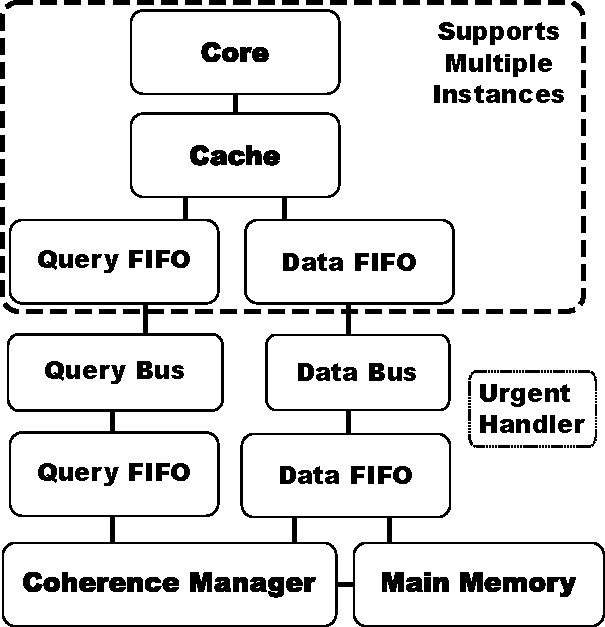
\includegraphics[width=0.7\textwidth]{\chapterdirectory/figure/model_overview.pdf}
\caption{Overview of the Instantiated Model}
\label{fig:analysis:model}
\end{center}
\end{figure}

\begin{figure}[hbt!]
\begin{center}
\begin{subfigure}[t]{0.35\textwidth}
\centering
\begin{lstlisting}
{INSTR_STORE,  1, 0, 0},
{INSTR_STORE,  2, 0, 0},
{INSTR_LOAD,   1, 0, 0},
{INSTR_STORE,  1, 0, 0},
{INSTR_LOAD,   3, 0, 0},
{INSTR_STORE,  2, 0, 0},
{INSTR_LOAD,   1, 0, 0},
{INSTR_STORE,  1, 0, 0},
{INSTR_LOAD,   2, 0, 0},
{INSTR_STORE,  2, 0, 0},
{INSTR_END,    0, 0, 0}
\end{lstlisting}
\caption{Program Model for Core 1}
\label{fig:analysis:demo_prog1}
\end{subfigure}
\begin{subfigure}[t]{0.35\textwidth}
\centering
\begin{lstlisting}
{INSTR_STORE,  1, 0, 0},
{INSTR_STORE,  3, 0, 0},
{INSTR_LOAD,   3, 0, 0},
{INSTR_STORE,  2, 0, 0},
{INSTR_LOAD,   1, 0, 0},
{INSTR_STORE,  2, 0, 0},
{INSTR_LOAD,   3, 0, 0},
{INSTR_STORE,  1, 0, 0},
{INSTR_LOAD,   2, 0, 0},
{INSTR_STORE,  3, 0, 0},
{INSTR_END,    0, 0, 0}
\end{lstlisting}
\caption{Program Model for Core 2}
\label{fig:analysis:demo_prog2}
\end{subfigure}
\end{center}
\caption{Program Models}
\label{fig:analysis:demo_progs}
\end{figure}

The instantiated model chosen to illustrate the analyses of this chapter is
shown Figure~\ref{fig:analysis:model}. The model of each program can
be seen on Figure~\ref{fig:analysis:demo_progs}, with \lstinline!Core1! running
the program from Figure~\ref{fig:analysis:demo_prog1} and \lstinline!Core2! the
one from Figure~\ref{fig:analysis:demo_prog2}. The model uses its default
parameters, as listed in Figure~\ref{fig:analysis:demo_params}. It uses the
MESI protocol from Section~\ref{sec:identification:mesi}.

Instantiated models still allow many different executions. For example, the
order in which caches access the query bus remain undecided, leaving all
possible combinations as a source of divergence between valid executions. These
valid executions are analyzed using of model checking, providing information on
the modeled system. In effect, each analysis is made of a number of formulas
written using the syntax detailed in Section~\ref{sec:uppaal_queries}. The
result of each analysis is an interpretation of the results of these model
checking queries.

\paragraph{WCET Analysis}~~\\
In Section~\ref{sec:analysis:wcet}, analyses are made on the instantiated model
to seek worst-case program execution times. The first result taken from these
analyses is the execution time of each program with cache coherence taken into
account. While deviating from interference analysis, this also makes it
possible to compare architecture configurations (see
Definition~\ref{def:configuration}) and their respective slowdown factors
(see Definition~\ref{def:slowdown-factor}).
There is a particular configuration which should be studied regardless of its
validity on the real system: running the programs without any shared variables.
While this result is likely to be of use on its own, comparing it with the
results from the analysis that has shared variables quantifies the impact of
interference on the execution time of the programs.

With knowledge only about program execution times, the applicant would not be
sufficiently informed to address the issue of cache coherence interference.
As a result, the other analyses focus on program instructions. Namely, how
interference affects them, and how they generate interference.

\paragraph{Hit \& Miss Analysis}~~\\
Section~\ref{sec:analysis:hit_and_miss} uses the instantiated model to
categorize each of the programs' instruction according to whether it finds the
memory element in the cache or not (cache hit or cache miss, referred to as
\textit{accuracy} thorough this chapter). This provides the user with an
understanding of which instructions are likely to have been impacted by cache
coherence and points out which ones have execution times that may vary because
of it. An auxiliary analysis looks at the accuracy of memory elements, which
might point out particularly troublesome memory elements.

\paragraph{Interference Categorization}~~\\
These accuracy analyses do not properly expose cache coherence interference.
Indeed, while the effects of the interference are found within the
categorization of instruction accuracy, the causes of the interference are not.
Section~\ref{sec:analysis:exposing_interference} proposes a categorization of
the effects of cache coherence interference. This makes it possible to annotate
the cache coherence protocol with the transitions that can cause interference
and the type of interference they generate.

\paragraph{Instruction Impact Analysis}~~\\
Using this annotated cache coherence protocol and the instantiated model,
Section~\ref{sec:analysis:missing_link} describes analyses that point out to
the applicant exactly which instructions can generate interference, what
category of interference they generate, which instructions can be affected, and
whether this occurs on all possible executions or only some of them. This
provides the information on instructions that was missing from the
analyses of Section~\ref{sec:analysis:hit_and_miss} and thus expose all cache
coherence interference to the applicant with sufficient details to be the basis
on which mitigation can be planned.
%This chapter illustrates its concepts by applying them to the model presented in
%this section. This model is an instance of the model presented in
%Chapter~\ref{cha:modeling_cache_coherence}, and is not based on any existing
%architecture, in order to keep the analysis results small enough to be easily
%understood.
